% Options for packages loaded elsewhere
\PassOptionsToPackage{unicode}{hyperref}
\PassOptionsToPackage{hyphens}{url}
%
\documentclass[
  12pt,
]{article}
\usepackage{lmodern}
\usepackage{amssymb,amsmath}
\usepackage{ifxetex,ifluatex}
\ifnum 0\ifxetex 1\fi\ifluatex 1\fi=0 % if pdftex
  \usepackage[T1]{fontenc}
  \usepackage[utf8]{inputenc}
  \usepackage{textcomp} % provide euro and other symbols
\else % if luatex or xetex
  \usepackage{unicode-math}
  \defaultfontfeatures{Scale=MatchLowercase}
  \defaultfontfeatures[\rmfamily]{Ligatures=TeX,Scale=1}
\fi
% Use upquote if available, for straight quotes in verbatim environments
\IfFileExists{upquote.sty}{\usepackage{upquote}}{}
\IfFileExists{microtype.sty}{% use microtype if available
  \usepackage[]{microtype}
  \UseMicrotypeSet[protrusion]{basicmath} % disable protrusion for tt fonts
}{}
\makeatletter
\@ifundefined{KOMAClassName}{% if non-KOMA class
  \IfFileExists{parskip.sty}{%
    \usepackage{parskip}
  }{% else
    \setlength{\parindent}{0pt}
    \setlength{\parskip}{6pt plus 2pt minus 1pt}}
}{% if KOMA class
  \KOMAoptions{parskip=half}}
\makeatother
\usepackage{xcolor}
\IfFileExists{xurl.sty}{\usepackage{xurl}}{} % add URL line breaks if available
\IfFileExists{bookmark.sty}{\usepackage{bookmark}}{\usepackage{hyperref}}
\hypersetup{
  pdftitle={Voting in a Pandemic: COVID-19 and Primary Turnout in Milwaukee, Wisconsin},
  pdfauthor={Kevin Morris; Peter Miller},
  hidelinks,
  pdfcreator={LaTeX via pandoc}}
\urlstyle{same} % disable monospaced font for URLs
\usepackage[margin = 1in]{geometry}
\usepackage{longtable,booktabs}
% Correct order of tables after \paragraph or \subparagraph
\usepackage{etoolbox}
\makeatletter
\patchcmd\longtable{\par}{\if@noskipsec\mbox{}\fi\par}{}{}
\makeatother
% Allow footnotes in longtable head/foot
\IfFileExists{footnotehyper.sty}{\usepackage{footnotehyper}}{\usepackage{footnote}}
\makesavenoteenv{longtable}
\usepackage{graphicx}
\makeatletter
\def\maxwidth{\ifdim\Gin@nat@width>\linewidth\linewidth\else\Gin@nat@width\fi}
\def\maxheight{\ifdim\Gin@nat@height>\textheight\textheight\else\Gin@nat@height\fi}
\makeatother
% Scale images if necessary, so that they will not overflow the page
% margins by default, and it is still possible to overwrite the defaults
% using explicit options in \includegraphics[width, height, ...]{}
\setkeys{Gin}{width=\maxwidth,height=\maxheight,keepaspectratio}
% Set default figure placement to htbp
\makeatletter
\def\fps@figure{htbp}
\makeatother
\setlength{\emergencystretch}{3em} % prevent overfull lines
\providecommand{\tightlist}{%
  \setlength{\itemsep}{0pt}\setlength{\parskip}{0pt}}
\setcounter{secnumdepth}{5}
\usepackage{rotating}
\usepackage{setspace}
\usepackage{booktabs}
\usepackage{longtable}
\usepackage{array}
\usepackage{multirow}
\usepackage{wrapfig}
\usepackage{float}
\usepackage{colortbl}
\usepackage{pdflscape}
\usepackage{tabu}
\usepackage{threeparttable}
\usepackage{threeparttablex}
\usepackage[normalem]{ulem}
\usepackage{makecell}
\usepackage{xcolor}
\newlength{\cslhangindent}
\setlength{\cslhangindent}{1.5em}
\newenvironment{cslreferences}%
  {\setlength{\parindent}{0pt}%
  \everypar{\setlength{\hangindent}{\cslhangindent}}\ignorespaces}%
  {\par}

\title{Voting in a Pandemic: COVID-19 and Primary Turnout in Milwaukee, Wisconsin}
\author{Kevin Morris\footnote{Researcher, Brennan Center for Justice at NYU School of Law, 120 Broadway Ste 1750, New York, NY 10271 (\href{mailto:kevin.morris@nyu.edu}{\nolinkurl{kevin.morris@nyu.edu}})} \and Peter Miller\footnote{Researcher, Brennan Center for Justice at NYU School of Law, 120 Broadway Ste 1750, New York, NY 10271 (\href{mailto:peter.miller@nyu.edu}{\nolinkurl{peter.miller@nyu.edu}})}}
\date{June 30, 2020}

\begin{document}
\maketitle
\begin{abstract}
We report the first study of the effect of the novel coronavirus SARS-CoV-2 (COVID-19) on voting behavior. We draw upon individual-level observations from Milwaukee matched to similar observations in the surrounding counties to assess whether fewer polling places in the primary election decreased turnout in the city. We find polling place consolidation reduced overall turnout by about 8.5 points and reduced turnout among the black population in the city by about 10.2 points. This effect becomes more pronounced as the distance between treated and control observations on either side of the municipal boundary increases, suggestive that COVID-19 itself reduced turnout separate from polling place consolidation. We conclude on the basis of these data that conversion to widespread absentee voting in the general election will result in disenfranchisement, which may be particularly marked among racial minorities.
\end{abstract}

\pagenumbering{gobble}
\pagebreak

\pagenumbering{arabic}
\doublespacing

The Wisconsin primary election provides a valuable means to assess how the novel coronavirus SARS-CoV-2 (COVID-19) has altered voting behavior in a natural experiment. We draw upon individual-level observations from Milwaukee and the surrounding suburban counties to assess whether fewer polling places in the election decreased turnout in the city. We find significant evidence for the claim, and this effect is larger in magnitude among minority populations.

The weeks leading up to the Wisconsin primary election on April 7 were tumultuous. Democratic Governor Tony Evers declared a state of emergency on March 12 when there were 8 confirmed COVID-19 cases.\footnote{See \url{https://www.dhs.wisconsin.gov/covid-19/cases.htm}.} On March 17, Evers issued a ban on all gatherings of more than 10 people.\footnote{See \url{https://evers.wi.gov/Documents/COVID19/UPDATEDOrder10People.pdf}.} On March 27, Evers called for every voter in the state to be sent an absentee ballot (Wise \protect\hyperlink{ref-Wise2020}{2020}). The Republican-controlled legislature refused this initiative. The weekend before the election, Evers called an emergency session of the legislature hoping to postpone the date of the election. This effort, too, was rebuffed. As a last resort, Evers issued an executive order on April 6 to delay the primary election until June 9\footnote{See \url{https://bit.ly/3fJTqZT}.} which was overturned by the state supreme court.\footnote{See \url{https://wapo.st/2Cg79sK}.} The U.S. Supreme Court also ruled absentee ballots would be invalid if the ballot was not hand-delivered by April 7 or postmarked by election day and received by April 13.\footnote{See \url{https://www.supremecourt.gov/opinions/19pdf/19a1016_o759.pdf}.}

These judicial maneuvers occurred against the backdrop of overstretched electoral resources. The \emph{Milwaukee Journal Sentinel} observed the state was short some 7 thousand poll workers on March 31 (Marley and Beck \protect\hyperlink{ref-Marley2020}{2020}). The reduction in polling places was acute in Milwaukee. Five polling places remained open, compared with 182 in November of 2016.\footnote{See \url{https://elections.wi.gov/elections-voting/2016/fall} and \url{https://elections.wi.gov/node/6524}.} Even as polling places were consolidated, a surge in absentee voting occurred. While 831 thousand ballots were cast by mail in the 2016 \emph{general election}, more than 1.09 million mail ballots were returned in the primary this year.\footnote{See \url{https://elections.wi.gov/index.php/node/4414} and \url{https://elections.wi.gov/node/6847}.} Nonetheless, there is evidence for ``leaked'' absentee ballots (Stewart \protect\hyperlink{ref-Stewart2010}{2010}): only 84.8\% of mail ballots delivered to voters were ultimately returned in time to be counted.

\hypertarget{prior-literature}{%
\subsubsection*{Prior Literature}\label{prior-literature}}
\addcontentsline{toc}{subsubsection}{Prior Literature}

Disrupting one's routine with regard to voting -- whether by relocating or reducing the number of polling places -- reduces turnout by imposing new search and transportation costs on voters (Brady and Mcnulty \protect\hyperlink{ref-Brady2011}{2011}). A moved polling place reduced the likelihood of voting by about 5.5 points in a 2001 local election (Haspel and Knotts \protect\hyperlink{ref-Haspel2005}{2005}). Consolidation between 2000 and 2008 reduced county-level turnout by about nine-tenths of a point (Kropf and Kimball \protect\hyperlink{ref-Kropf2012}{2012}, 68). Increasing the distance to polls in California in 2003 reduced the likelihood of voting at the polls by between 2 and 4 points. Absentee voting is more likely as the distance to the polls increases, but this effect is not large enough to offset the decrease from consolidation itself (Brady and Mcnulty \protect\hyperlink{ref-Brady2011}{2011}). Consolidating polling places in a New York State local election reduced turnout by an average of 7 points (McNulty, Dowling, and Ariotti \protect\hyperlink{ref-McNulty2009}{2009}). A recent study of nine municipalities in Massachusetts and Minnesota found increasing the distance to the polls by about one-quarter mile reduces turnout by between 2 and 5 points, and that this effect is more pronounced among ``high-minority, ­low-income, and low-car-availability areas'' in the context of a non-presidential election (Cantoni \protect\hyperlink{ref-Cantoni2020}{2020}, 88).

The effect of distance to the polling place on voting is nonlinear (Dyck and Gimpel \protect\hyperlink{ref-Dyck2005}{2005}, 541--42; Gimpel and Schuknecht \protect\hyperlink{ref-Gimpel2003}{2003}, 481--84). Dyck and Gimpel (\protect\hyperlink{ref-Dyck2005}{2005}) deploy observations ranging from .1 to 65 miles from the polling place. They report being one standard deviation from the polls (about 1.75 miles) reduces the likelihood of voting at the polls by 2.3 points, but makes absentee voting more likely by 0.9 points. A study of three counties in Maryland in the 2000 election finds moving 1 mile \emph{closer} to the polls makes voting \emph{more} likely by 0.45 points, while observing generally ``{[}t{]}urnout is highest when distances to the polling place are very short, and when they are excessively long, but lower in the middling ranges of distance'' (Gimpel and Schuknecht \protect\hyperlink{ref-Gimpel2003}{2003}, 481).

\hypertarget{data-and-research-design}{%
\subsubsection*{Data and Research Design}\label{data-and-research-design}}
\addcontentsline{toc}{subsubsection}{Data and Research Design}

We use individual-level voter registration and turnout records from L2 Political to estimate all our models. In addition to providing the information available in the registered voter file, L2 provides estimates for voters' partisan affiliation (voters do not register with parties in Wisconsin), race, household income, and education. L2 also geocodes voters to their home addresses. The data indicates whether someone voted, but not vote mode. That we find negative treatment effects indicates that increased absentee voting did not \emph{entirely} offset the effect of polling place consolidation.

Although Milwaukee reduced the total number of polling places, the rest of the state did not see such drastic consolidation. Outside of Milwaukee, the state had 10.2\% fewer polling places open in April 2020 than November 2016. However, residents of Milwaukee were also likely subjected to a \emph{second} treatment due to the severity of COVID-19. In Milwaukee County there had been roughly 14 positive tests for COVID-19 per 10,000 residents as of the date of the primary election, compared with 7.5 positive tests per 10,000 residents in Ozaukee County, and 4.4, 4.2, and 3.4 in Washington, Waukesha, and Racine Counties, respectively.\footnote{See \url{https://www.dhs.wisconsin.gov/covid-19/county.htm}.} Simply comparing the turnout of Milwaukee to the suburbs therefore cannot reveal the depressive effect of polling place consolidation alone, but rather the net effect of higher exposure to the pandemic and the consolidation of polling places.

To isolate the effect of polling place consolidation from COVID-19, we leverage electoral jurisdiction boundaries as an assignment to treatment mechanism (Kaplan and Yuan \protect\hyperlink{ref-Kaplan2020}{2020}; Cantoni \protect\hyperlink{ref-Cantoni2020}{2020}). Our primary design is a regression discontinuity in space that exploits the municipal boundary line to compare turnout for voters on either side of the ``cutpoint'' boundary (Keele, Titiunik, and Zubizarreta \protect\hyperlink{ref-Keele2015}{2015}). Research from New Orleans indicates that COVID-19 is clustered at the neighborhood level (van Holm, Wyczalkowski, and Dantzler \protect\hyperlink{ref-vanHolm2020}{2020}), and we therefore assume that voters who live in close proximity to one another but on either side of the boundary were exposed to similar experiences with COVID-19.

The traditional regression discontinuity framework, however, relies on the assumption that individuals cannot ``select'' around the cutpoint; in other words, that within a narrow window individuals on either side of the cutpoint are identical. That is perhaps too strong of an assumption. Voters very near one another but on opposite sides of the border might differ in meaningful ways. Keele, Titiunik, and Zubizarreta (\protect\hyperlink{ref-Keele2015}{2015}) offers one way of dealing with this problem: ``When there appears to be strong self-selection around the border of interest, one alternative is to combine designs and to assume that, after conditioning on covariates, treatment assignment is as-if randomized for those who live near the city limit'' (page 228). We adopt this approach by genetically matching (Sekhon \protect\hyperlink{ref-Sekhon2009}{2009}, \protect\hyperlink{ref-Sekhon2011}{2011}) each registered voter in Milwaukee City to two voters who live outside the city but in Milwaukee, Racine, Waukesha, Washington, or Ozaukee County.\footnote{Each of these counties shares a border with Milwaukee County. Treated and control voters are matched exactly on turnout in the 2016 and 2018 primary elections, and on their partisan affiliation. Voters are also matched on their gender, their household income, whether they have a college education, and their race / ethnicity. Voters are also matched on their latitude and longitude to ensure physical proximity to one another.} After the matching procedure has been completed, we test how the estimated treatment effect changes as we vary the maximum distance allowed between treated and control voters.

Although this differs from a regression discontinuity in which there is a band around a cutpoint, the logic is the same. As the maximum allowed distance between treated and control voters approaches zero, we are in fact reducing the band around the cutpoint represented by the municipal border. For instance, when the maximum distance allowed between a treated voter and her match is 0.5 miles, each voter will live (on average) within 0.25 miles of the border. It is important to note that this is more conservative than matching treated and control voters within a buffer around the border --- not only must pairs both live within a buffer, they must also live near one another \emph{within} that buffer. Just as narrowing the band allows us to home in on the effect of polling place closures, by expanding the maximum allowed distance we can estimate the net effect of polling place consolidation plus Milwaukee City's increased exposure to COVID-19.

This set-up allows us to test two hypotheses:

Hypothesis A: When the maximum distance allowed between treated and control voters approaches zero, voters in Milwaukee will have turned out at a lower rate than their controls just over the municipal border. This effect will be considered the effect of consolidated polling places.\footnote{Insofar as some of the suburban municipalities closed some polling places, any treatment effect will be biased towards zero, thus making our estimates conservative.}

Hypothesis B: As we allow the maximum allowed distance to increase, the negative treatment effect will grow larger. We expect that the worse effects of COVID-19 depressed turnout above-and-beyond the effects of consolidated polling places in Milwaukee City.

\hypertarget{results}{%
\subsubsection*{Results}\label{results}}
\addcontentsline{toc}{subsubsection}{Results}

Our matching procedure is successful: we achieve 100 percent improvement in the mean difference between treated and control voters along 9 of our 11 (excluding longitude and latitude) covariates. The other two --- household income and share male --- improve by more than 99.95\%. Treated voters and their matched controls live an average of 2.5 miles apart.

Table \ref{tab:reg-table} presents the results of ordinary least squares regressions testing the treatment effect. In Table \ref{tab:reg-table} we require treated and control voters to live within 0.5 miles of one another.\footnote{A treated voter might live within the cutoff distance from one of her controls but not the other. The regression weights are updated for each regression to reflect this possibility.} The dependent variable takes the value 1 if a voter cast a ballot in the April primary, and 0 if she did not. We also test whether the treatment effect was different for Black voters than for other voters which Cantoni (\protect\hyperlink{ref-Cantoni2020}{2020}) indicates is possible. Models 1 and 3 include just the treatment variable (and, in Model 3, the interaction term) while Models 2 and 4 add in the variables on which the matching was performed (but without latitude and longitude). Robust standard errors are clustered at the level of the match (Abadie and Spiess \protect\hyperlink{ref-Abadie2019}{2019}).

\begin{singlespace}

\input{"../temp/reg.tex"}
\end{singlespace}

Models 1 and 2 indicate that turnout was depressed by roughly 8.6 percentage points in the April primary in Milwaukee City relative to suburban voters. Models 3 and 4 indicate that this decrease was especially pronounced among Black voters, who saw turnout nearly 10.2 percentage points below that of their suburban matches. Because of the tight geographic restriction imposed here, we argue that this represents the causal effect of polling place consolidation. This is a large treatment effect, and supports our Hypothesis A.

We are also interested in whether the findings hold when we relax the geographic assumption by further restricting the maximum allowed distance, and also in whether the size of the treatment effect grows as we include pairs who live further away from one another. Figure \ref{fig:coef-plot} re-estimates of Model 3 from Table \ref{tab:reg-table} using different maximum distances between treated and control voters.\footnote{The interaction effect becomes non-significant at the narrowest bands, though it remains negative. This is probably due more to the fact that very few treated Black voters lived near the municipal border and had matches just on the other side; in our most conservative pool, we have just 82 treated Black voters, while Black voters make up just 5\% of the treated voters in the 0.25-mile model. In an alternative model, where we match all Milwaukee voters within 0.125 of the boundary to suburban voters within the same distance of the boundary, we maintain excellent covariate matches and the interaction effect is significant at the 99\% confidence level. The coefficient on Black × Lives in Milwaukee in this model is -2.6 points.}

\begin{figure}[H]

{\centering 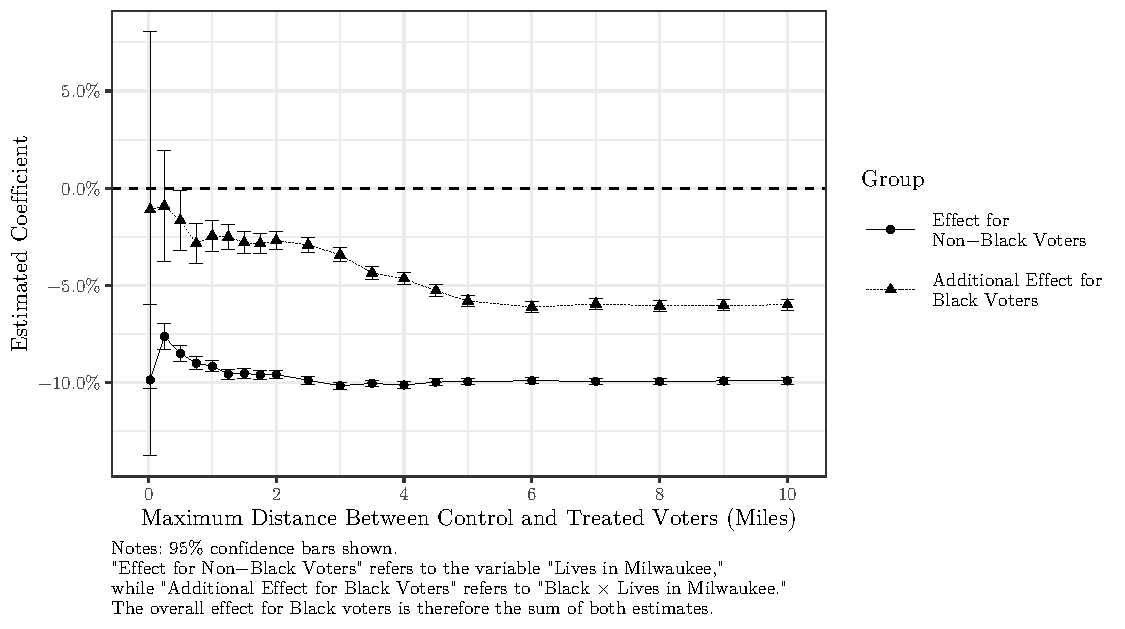
\includegraphics{mke_turnout_files/figure-latex/plot-1} 

}

\caption{\label{fig:coef-plot}Estimated Depressive Effect of Living in Milwaukee, 2020 Primary}\label{fig:plot}
\end{figure}

As we allow the maximum distance between treated and control voters to grow, the overall treatment effect and interaction effect grow in magnitude; turnout in Milwaukee was apparently depressed by mechanisms above-and-beyond those explained by polling place consolidation and the voter demographics for which we controlled in the matching procedure. As discussed above, Milwaukee was hard-hit by the COVID-19 crisis; this analysis demonstrates that COVID-19 likely directly depressed turnout in Milwaukee City. The difference in overall treatment effect between the half-mile and most lenient models is roughly 1.4 percentage points (the interaction effect grows by 4.3 percentage points). Thus COVID-19 likely reduced turnout relative to the suburbs (through mechanisms other than polling place consolidation) by 1.4 percentage points for non-Black voters, and as much as 5.7 percentage points for Black voters. This provides evidence to support Hypothesis B.

\hypertarget{discussion}{%
\subsubsection*{Discussion}\label{discussion}}
\addcontentsline{toc}{subsubsection}{Discussion}

Polling place closures have long been understood to reduce turnout among voters. This note makes clear that polling place closures reduced turnout in the 2020 primary in Milwaukee in the context of COVID-19 and unprecedented demand for absentee ballots. While the effect was perhaps smaller than it would have been absent robust messaging about mail voting, the 8.6 percentage point decrease in a primary contest is still quite large (turnout among control voters was 26.1\%). We also find this demobilizing effect better described as logarithmically approaching a limit rather than the nonlinear effect found in prior studies. Troublingly, the depressive effect was larger for Black than for non-Black voters, raising concerns about racial representation in the November 2020 elections as jurisdictions shift to greater access to mail ballots. Whether this is because racial minorities are perhaps less likely to request mail ballots this year (Morris \protect\hyperlink{ref-Morris2020}{2020}), because their mail ballots are rejected at higher rates (Shino, Suttmann-Lea, and Smith \protect\hyperlink{ref-Shino2020}{2020}), or some combination of these factors is unclear and should be the focus of future research.

This note answers just one question related to the effect of COVID-19: given the pandemic, how do polling place closures affect turnout? Future research must consider the overall turnout and representational impacts of COVID-19 on this year's contests. The primary elections in Milwaukee, Wisconsin, make one thing clear, however: voters will not seamlessly transition to vote by mail, and polling place closures this fall will come at the expense of turnout --- particularly the turnout of Black Americans.

\newpage

\hypertarget{references}{%
\subsubsection*{References}\label{references}}
\addcontentsline{toc}{subsubsection}{References}

\hypertarget{refs}{}
\begin{cslreferences}
\leavevmode\hypertarget{ref-Abadie2019}{}%
Abadie, Alberto, and Jann Spiess. 2019. ``Robust Post-Matching Inference.'' \emph{Working Paper.}

\leavevmode\hypertarget{ref-Brady2011}{}%
Brady, Henry E., and John E. Mcnulty. 2011. ``Turning Out to Vote: The Costs of Finding and Getting to the Polling Place.'' \emph{American Political Science Review} 105 (1): 115--34. \url{https://doi.org/10.1017/S0003055410000596}.

\leavevmode\hypertarget{ref-Cantoni2020}{}%
Cantoni, Enrico. 2020. ``A Precinct Too Far: Turnout and Voting Costs.'' \emph{American Economic Journal: Applied Economics} 12 (1): 61--85.

\leavevmode\hypertarget{ref-Dyck2005}{}%
Dyck, Joshua, and James Gimpel. 2005. ``Distance, Turnout, and the Convenience of Voting.'' \emph{Social Science Quarterly} 86 (3): 531--48.

\leavevmode\hypertarget{ref-Gimpel2003}{}%
Gimpel, James, and Jason Schuknecht. 2003. ``Political Participation and the Accessibility of the Ballot Box.'' \emph{Political Geography} 22: 471--88.

\leavevmode\hypertarget{ref-Haspel2005}{}%
Haspel, Moshe, and H. Gibbs Knotts. 2005. ``Location, Location, Location: Precinct Placement and the Costs of Voting.'' \emph{Journal of Politics} 67 (2): 560--73.

\leavevmode\hypertarget{ref-vanHolm2020}{}%
Holm, Eric Joseph van, Christopher Wyczalkowski, and Prentiss Dantzler. 2020. ``Neighborhood Conditions and the Initial Outbreak of COVID-19: The Case of Louisiana.'' SSRN Scholarly Paper ID 3625990. Rochester, NY: Social Science Research Network.

\leavevmode\hypertarget{ref-Kaplan2020}{}%
Kaplan, Ethan, and Haishan Yuan. 2020. ``Early Voting Laws, Voter Turnout, and Partisan Vote Composition: Evidence from Ohio.'' \emph{American Economic Journal: Applied Economics} 12 (1): 32--60.

\leavevmode\hypertarget{ref-Keele2015}{}%
Keele, Luke, Rocío Titiunik, and José R. Zubizarreta. 2015. ``Enhancing a Geographic Regression Discontinuity Design Through Matching to Estimate the Effect of Ballot Initiatives on Voter Turnout.'' \emph{Journal of the Royal Statistical Society: Series A (Statistics in Society)} 178 (1): 223--39. \url{https://doi.org/10.1111/rssa.12056}.

\leavevmode\hypertarget{ref-Kropf2012}{}%
Kropf, Martha E., and David C. Kimball. 2012. \emph{Helping America Vote: The Limits of Election Reform}. New York ; London: Routledge.

\leavevmode\hypertarget{ref-Marley2020}{}%
Marley, Patrick, and Molly Beck. 2020. ``Lack of Poll Workers Across Wisconsin, Flood of Absentee Ballots Spark Fears Votes Will Go Uncounted.'' \emph{Milwaukee Journal Sentinel}, March 31, 2020. \url{https://www.jsonline.com/story/news/politics/elections/2020/03/31/coronavirus-wisconsin-tony-evers-asks-state-workers-staff-polls/5093547002/}.

\leavevmode\hypertarget{ref-McNulty2009}{}%
McNulty, John, Conor Dowling, and Margaret Ariotti. 2009. ``Driving Saints to Sin: How Increasing the Difficulty of Voting Dissuades Even the Most Motivated Voters.'' \emph{Political Analysis} 17 (4): 435--55.

\leavevmode\hypertarget{ref-Morris2020}{}%
Morris, Kevin. 2020. ``Who's Requesting Mail Ballots in Georgia's Upcoming Primary?'' Brennan Center for Justice. June 10, 2020. \url{https://www.brennancenter.org/our-work/research-reports/whos-requesting-mail-ballots-georgias-upcoming-primary}.

\leavevmode\hypertarget{ref-Sekhon2009}{}%
Sekhon, Jasjeet. 2009. ``Opiates for the Matches: Matching Methods for Causal Inference.'' \emph{Annual Review of Political Science} 12: 487--508.

\leavevmode\hypertarget{ref-Sekhon2011}{}%
Sekhon, Jasjeet S. 2011. ``Multivariate and Propensity Score Matching Software with Automated Balance Optimization: The Matching Package for R.'' \emph{Journal of Statistical Software} 42 (1): 1--52. \url{https://doi.org/10.18637/jss.v042.i07}.

\leavevmode\hypertarget{ref-Shino2020}{}%
Shino, Enrijeta, Mara Suttmann-Lea, and Daniel A. Smith. 2020. ``Analysis \textbar{} Here's the Problem with Mail-in Ballots: They Might Not Be Counted.'' Washington Post. May 21, 2020. \url{https://www.washingtonpost.com/politics/2020/05/21/heres-problem-with-mail-in-ballots-they-might-not-be-counted/}.

\leavevmode\hypertarget{ref-Stewart2010}{}%
Stewart, Charles. 2010. ``Losing Votes by Mail.'' \emph{New York University Journal of Legislation and Public Policy} 13: 573--602.

\leavevmode\hypertarget{ref-Wise2020}{}%
Wise, David. 2020. ``Evers Calls for All Voters to Be Mailed Absentee Ballots \textbar{} WisPolitics.Com.'' \emph{WisPolitics}, March 27, 2020. \url{https://www.wispolitics.com/2020/evers-calls-for-all-voters-to-be-mailed-absentee-ballots/}.
\end{cslreferences}

\end{document}
